
\chapter{Результаты}\label{chapt_results}
В результате полугода работы прибора ДЭПРОН накоплен большой массив данных - 25 тысяч файлов бинарных данных, общим объемом 100 МБайт. Первичные данные были распакованы и сохранены в текстовом виде 
Далее информация от прибора была визуализирована с помошью пакета \texttt{lattice} и базовой графической системы R. 
В первую очередь для каждого дня работы прибора были построены карты скоростей счета в детекторе 1\ref{sec:planetDose}. Аналогично картам были построены долготные зависимости скоростей счета в первом детекторе, эти графики позволили оперативно заметить резкие всплески потоков частиц во внешнем радиационном поясе. Также для каждого дня были построены карты скоростей счета в координатах МакИлвайна, 

\section{Планетарное распределение потоков частиц, мощности дозы на высоте полета КА а также потоков нейтронов} \label{sec:planetDose}


\section{Распределения мощности дозы в области ЮАА}

\section{Распределения мощности дозы в авроральных областях}
Приполярные области отличаются высокой вариабельностью потоков чатиц и соответственно доз. В основном повышенные потоки регистрируются в первом полупроводниковом детекторе, что говорит о 
При первичной обработке данных были построены графики 
\begin{figure}[h]
	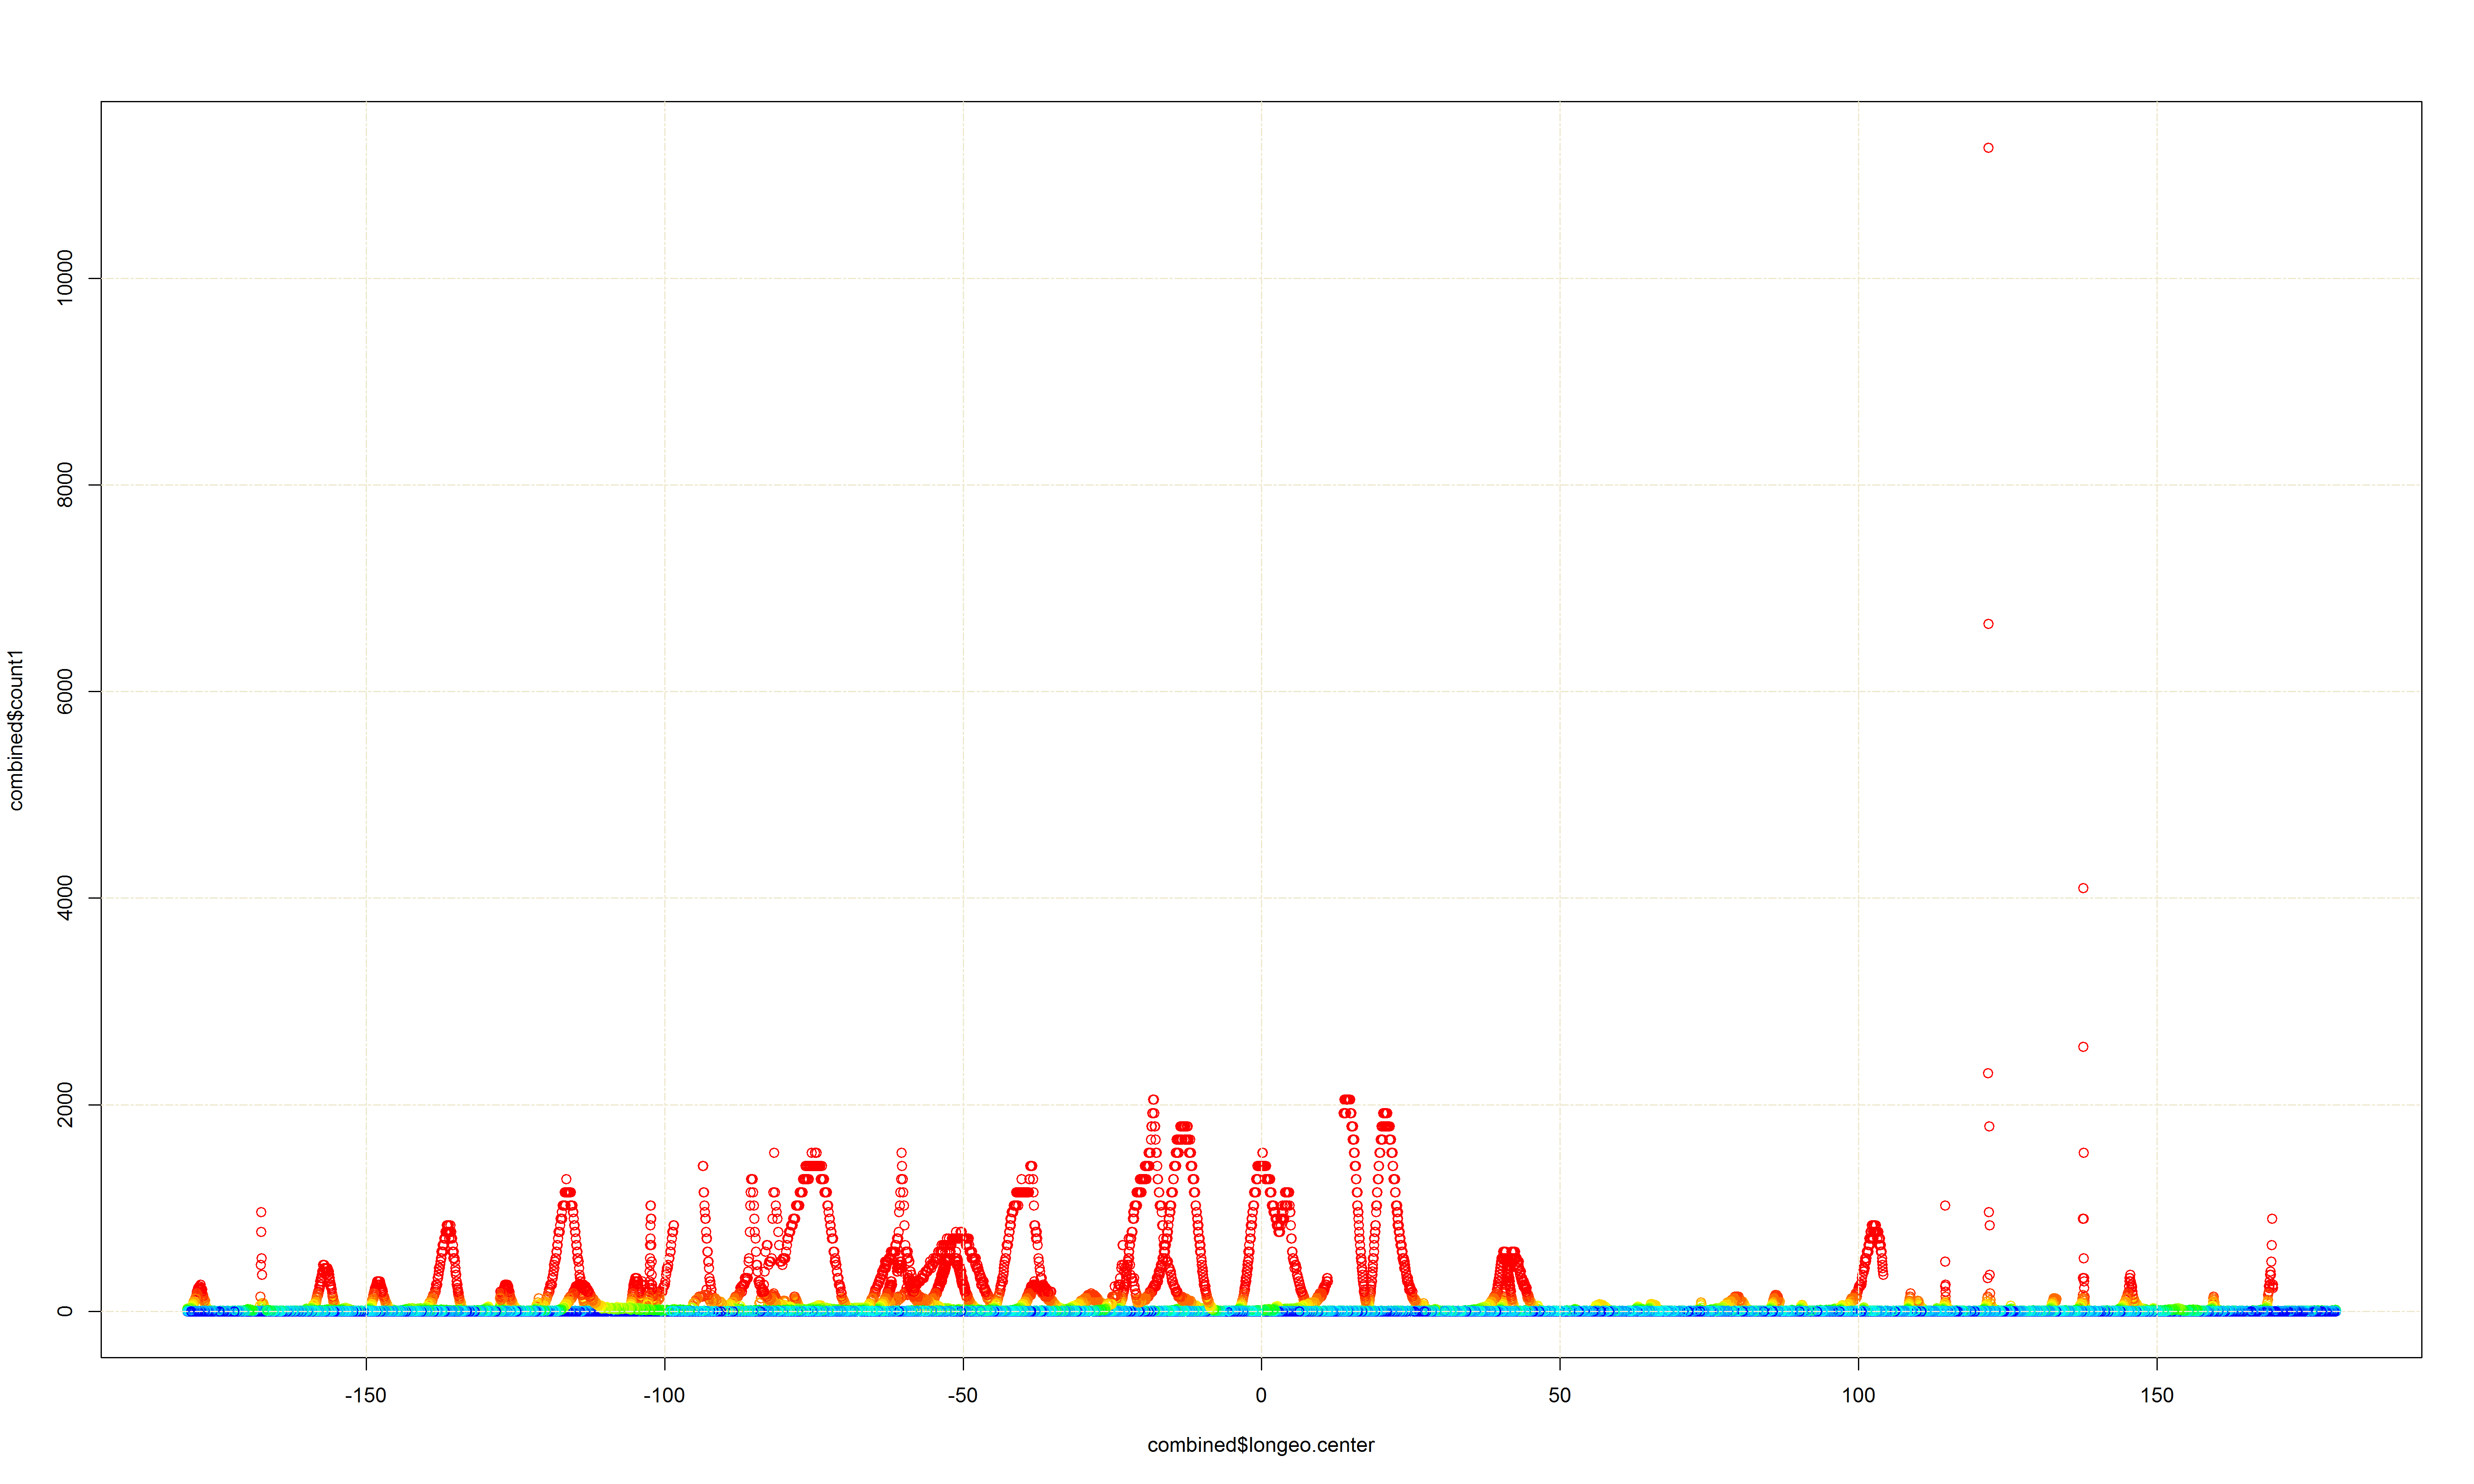
\includegraphics[width=0.8\linewidth]{images/Flash/depron_lat_map_148}
	\caption[Потокизаряженных частиц в детекторе 1]{}
	\caption{}
	\label{fig:depronlatmap148}
\end{figure}
Рассмотреть зависимости дозы в L-B координатах разделив при этом утреннее в вечернее местное магнитное время (MLT) о наличии магнитной бури следить по индексам A(e) A(l), причем по мнению Антоновой стоит выбрать спокойный период.

\begin{figure}
	\centering
	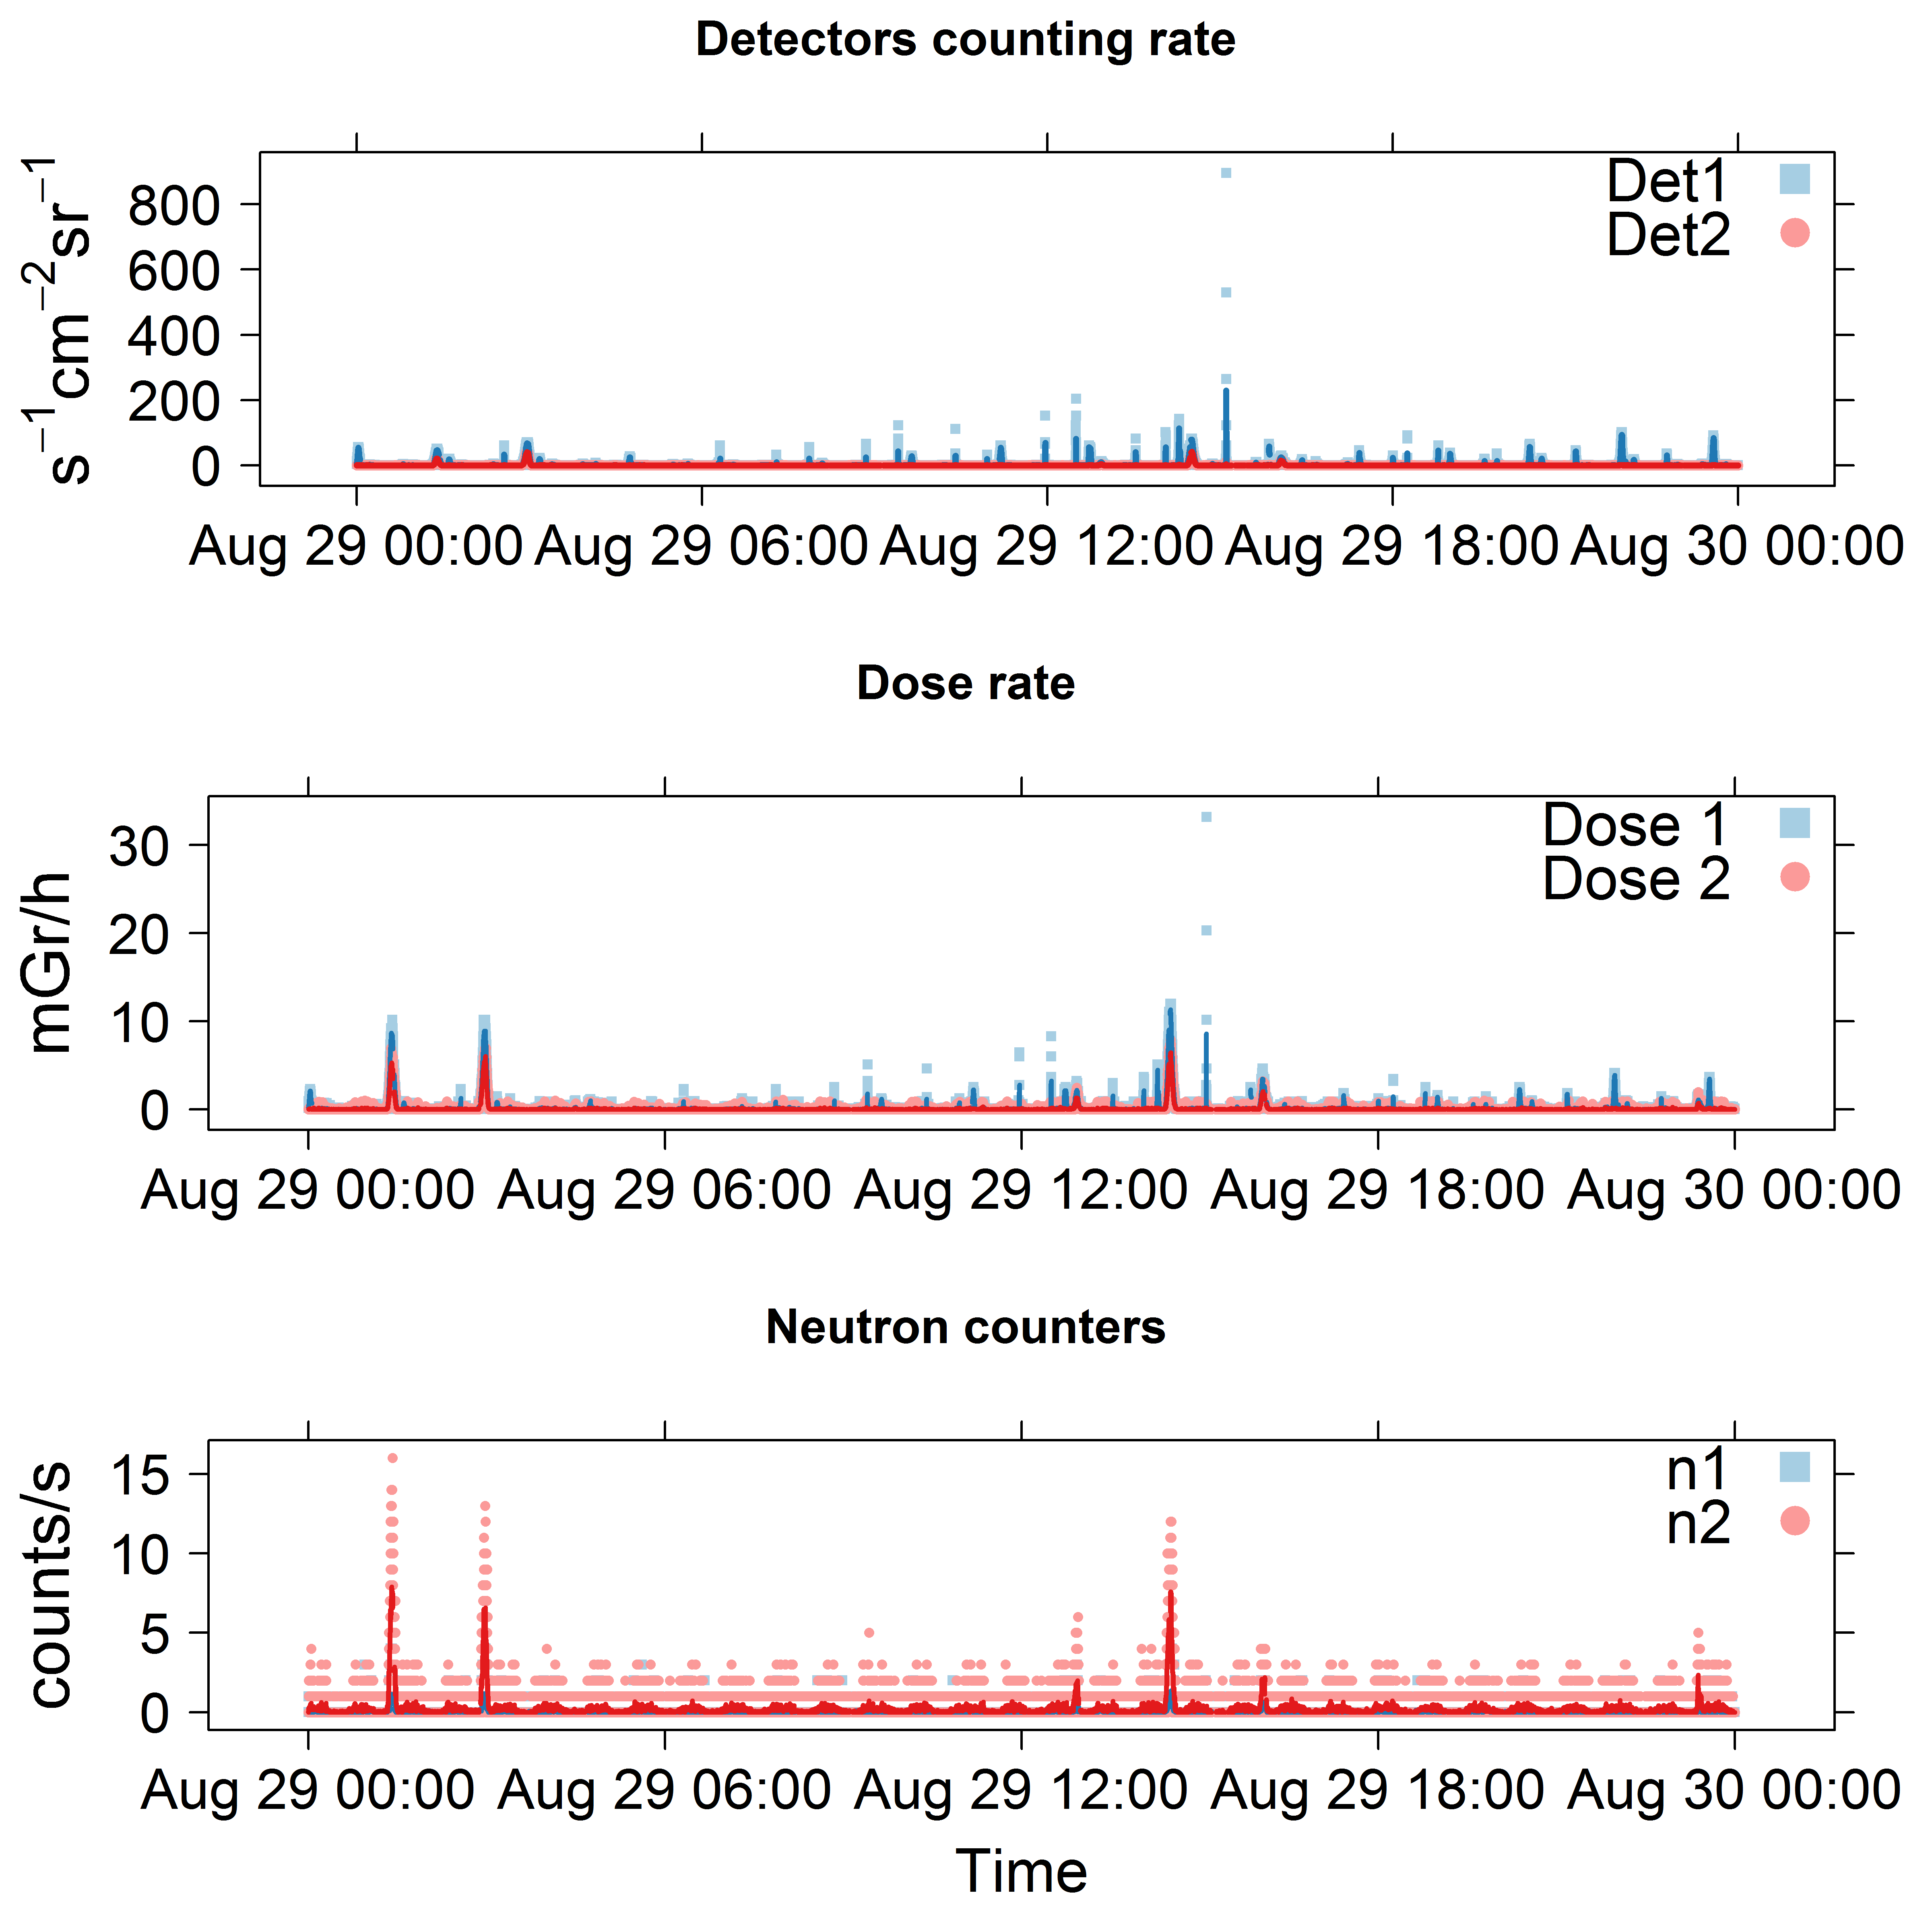
\includegraphics[width=0.7\linewidth]{images/results/depron_sec_log_new08-29-16}
	\caption{}
	\label{fig:depronseclognew08-29-16}
\end{figure}

\begin{figure}
	\centering
	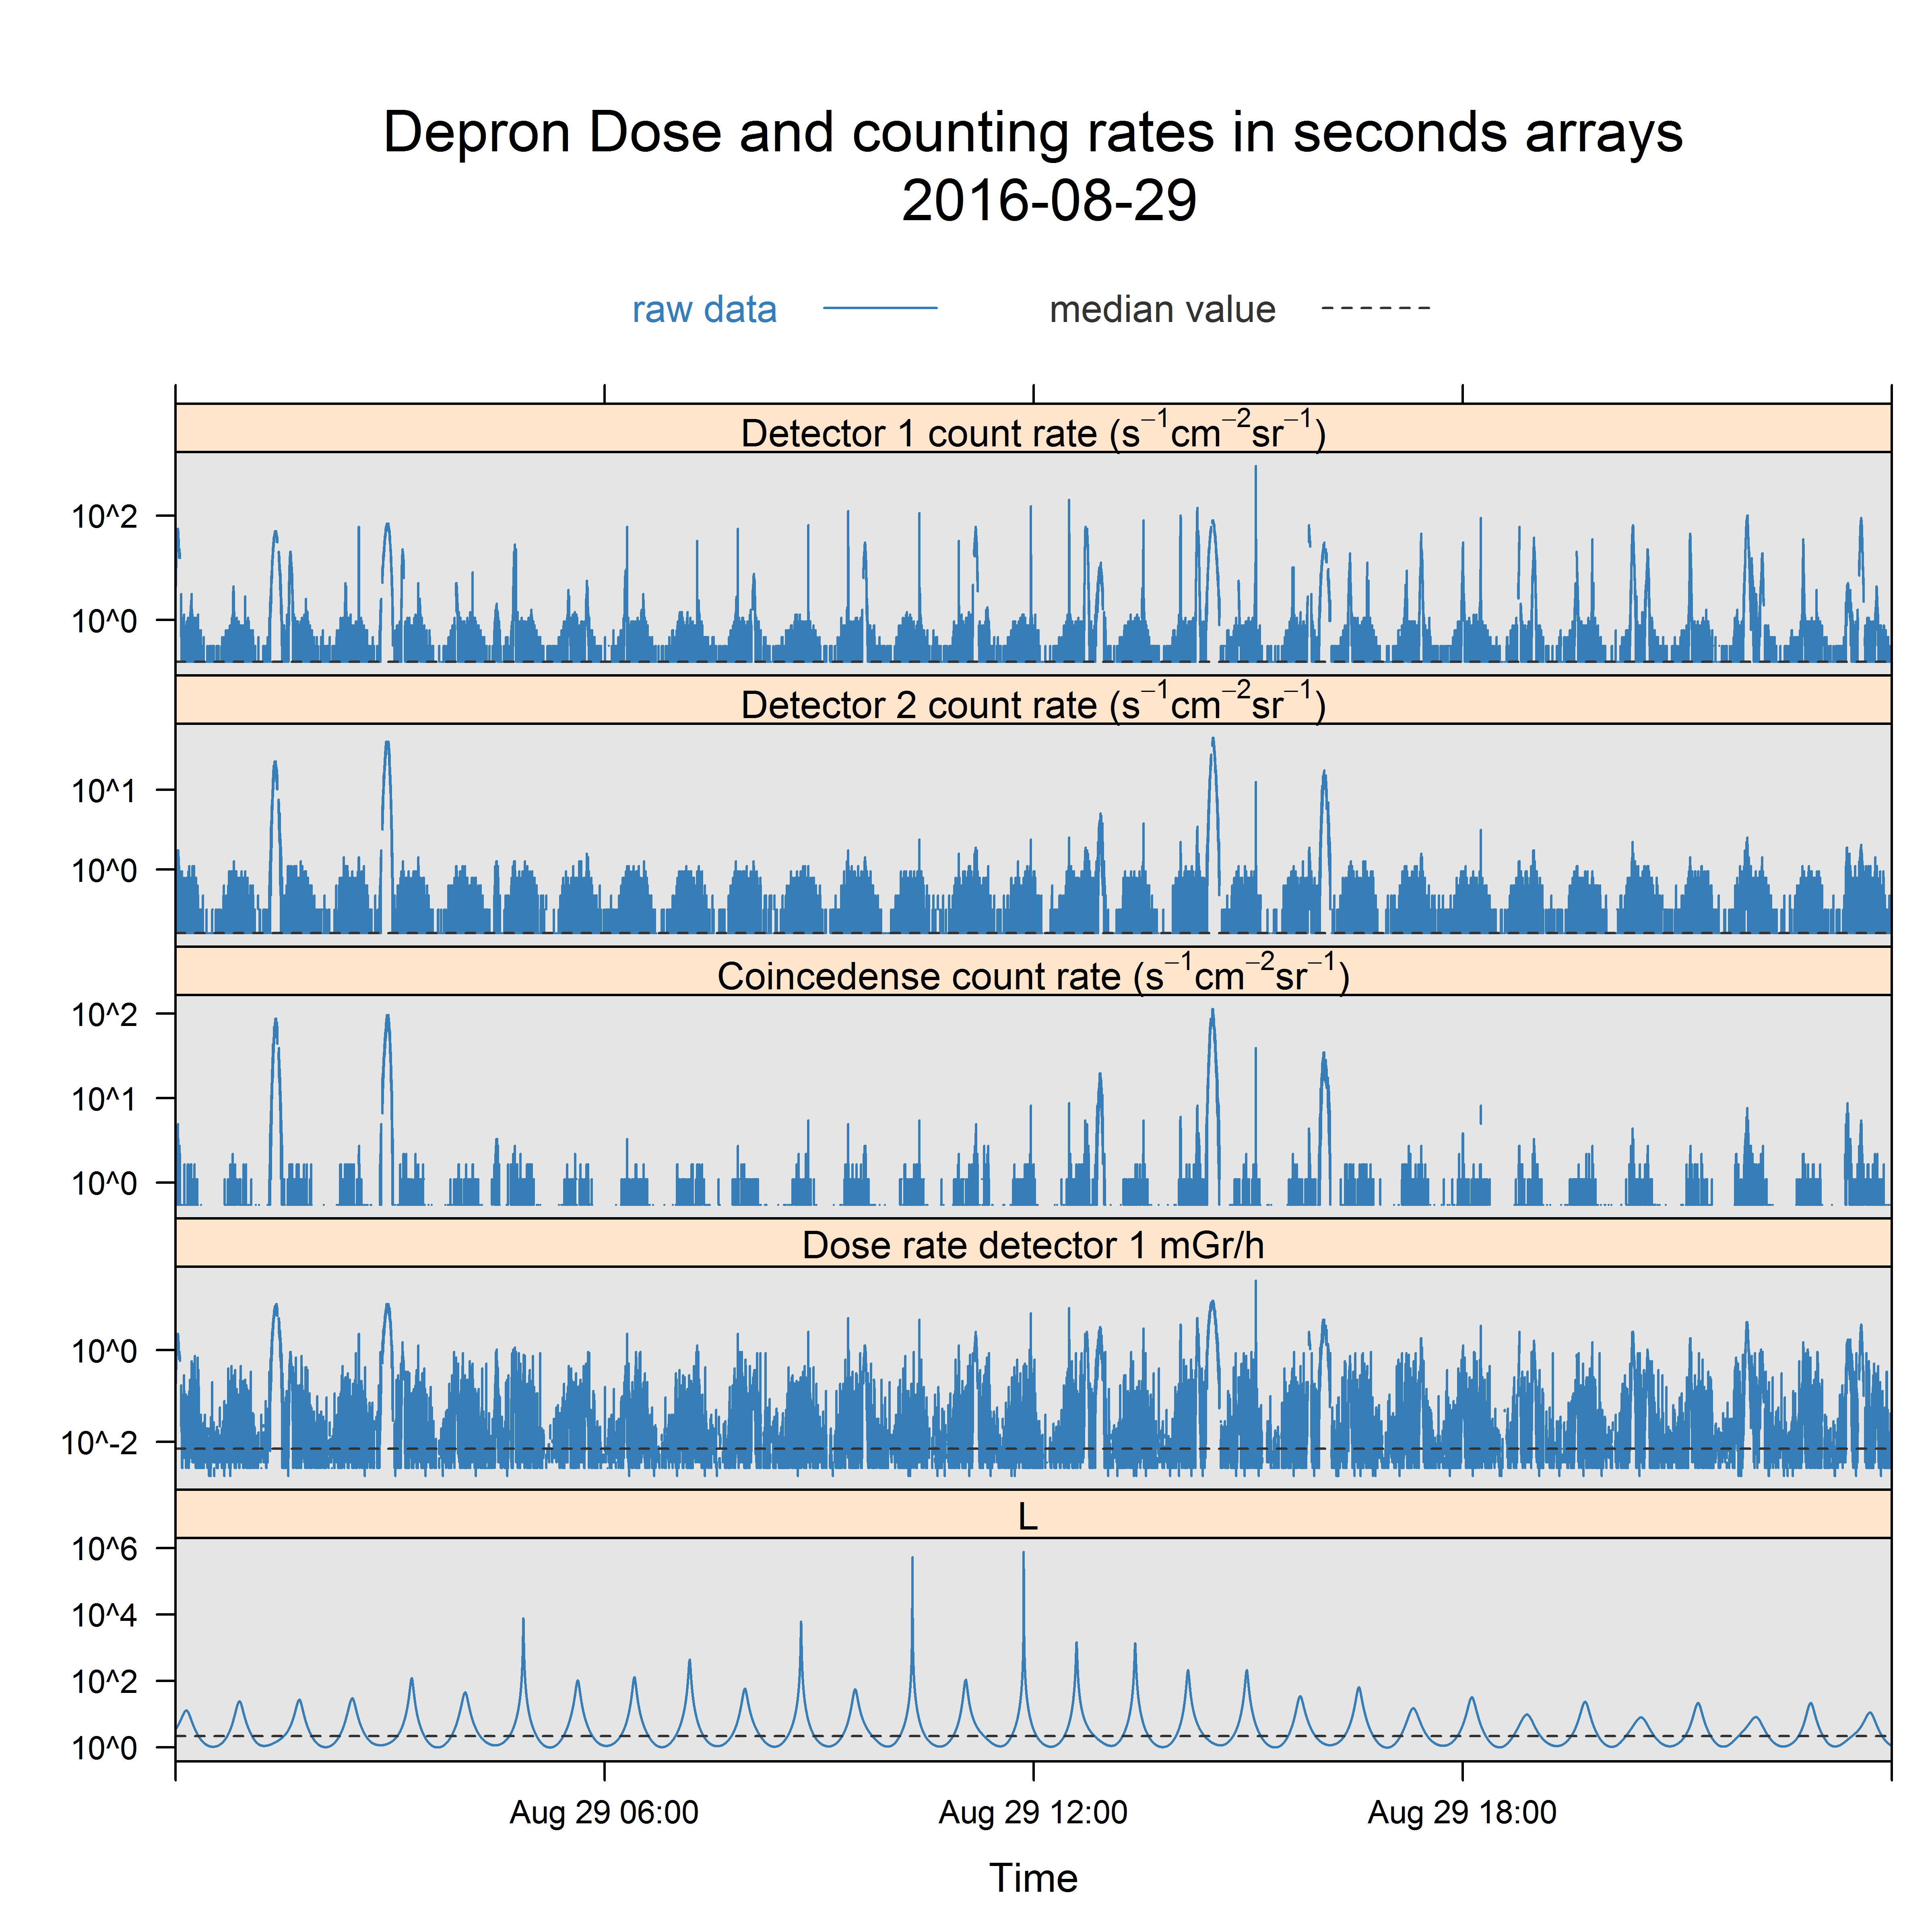
\includegraphics[width=0.7\linewidth]{images/results/depron_sec_log08-29-16}
	\caption{}
	\label{fig:depronseclog08-29-16}
\end{figure}



\begin{figure}
	\centering
	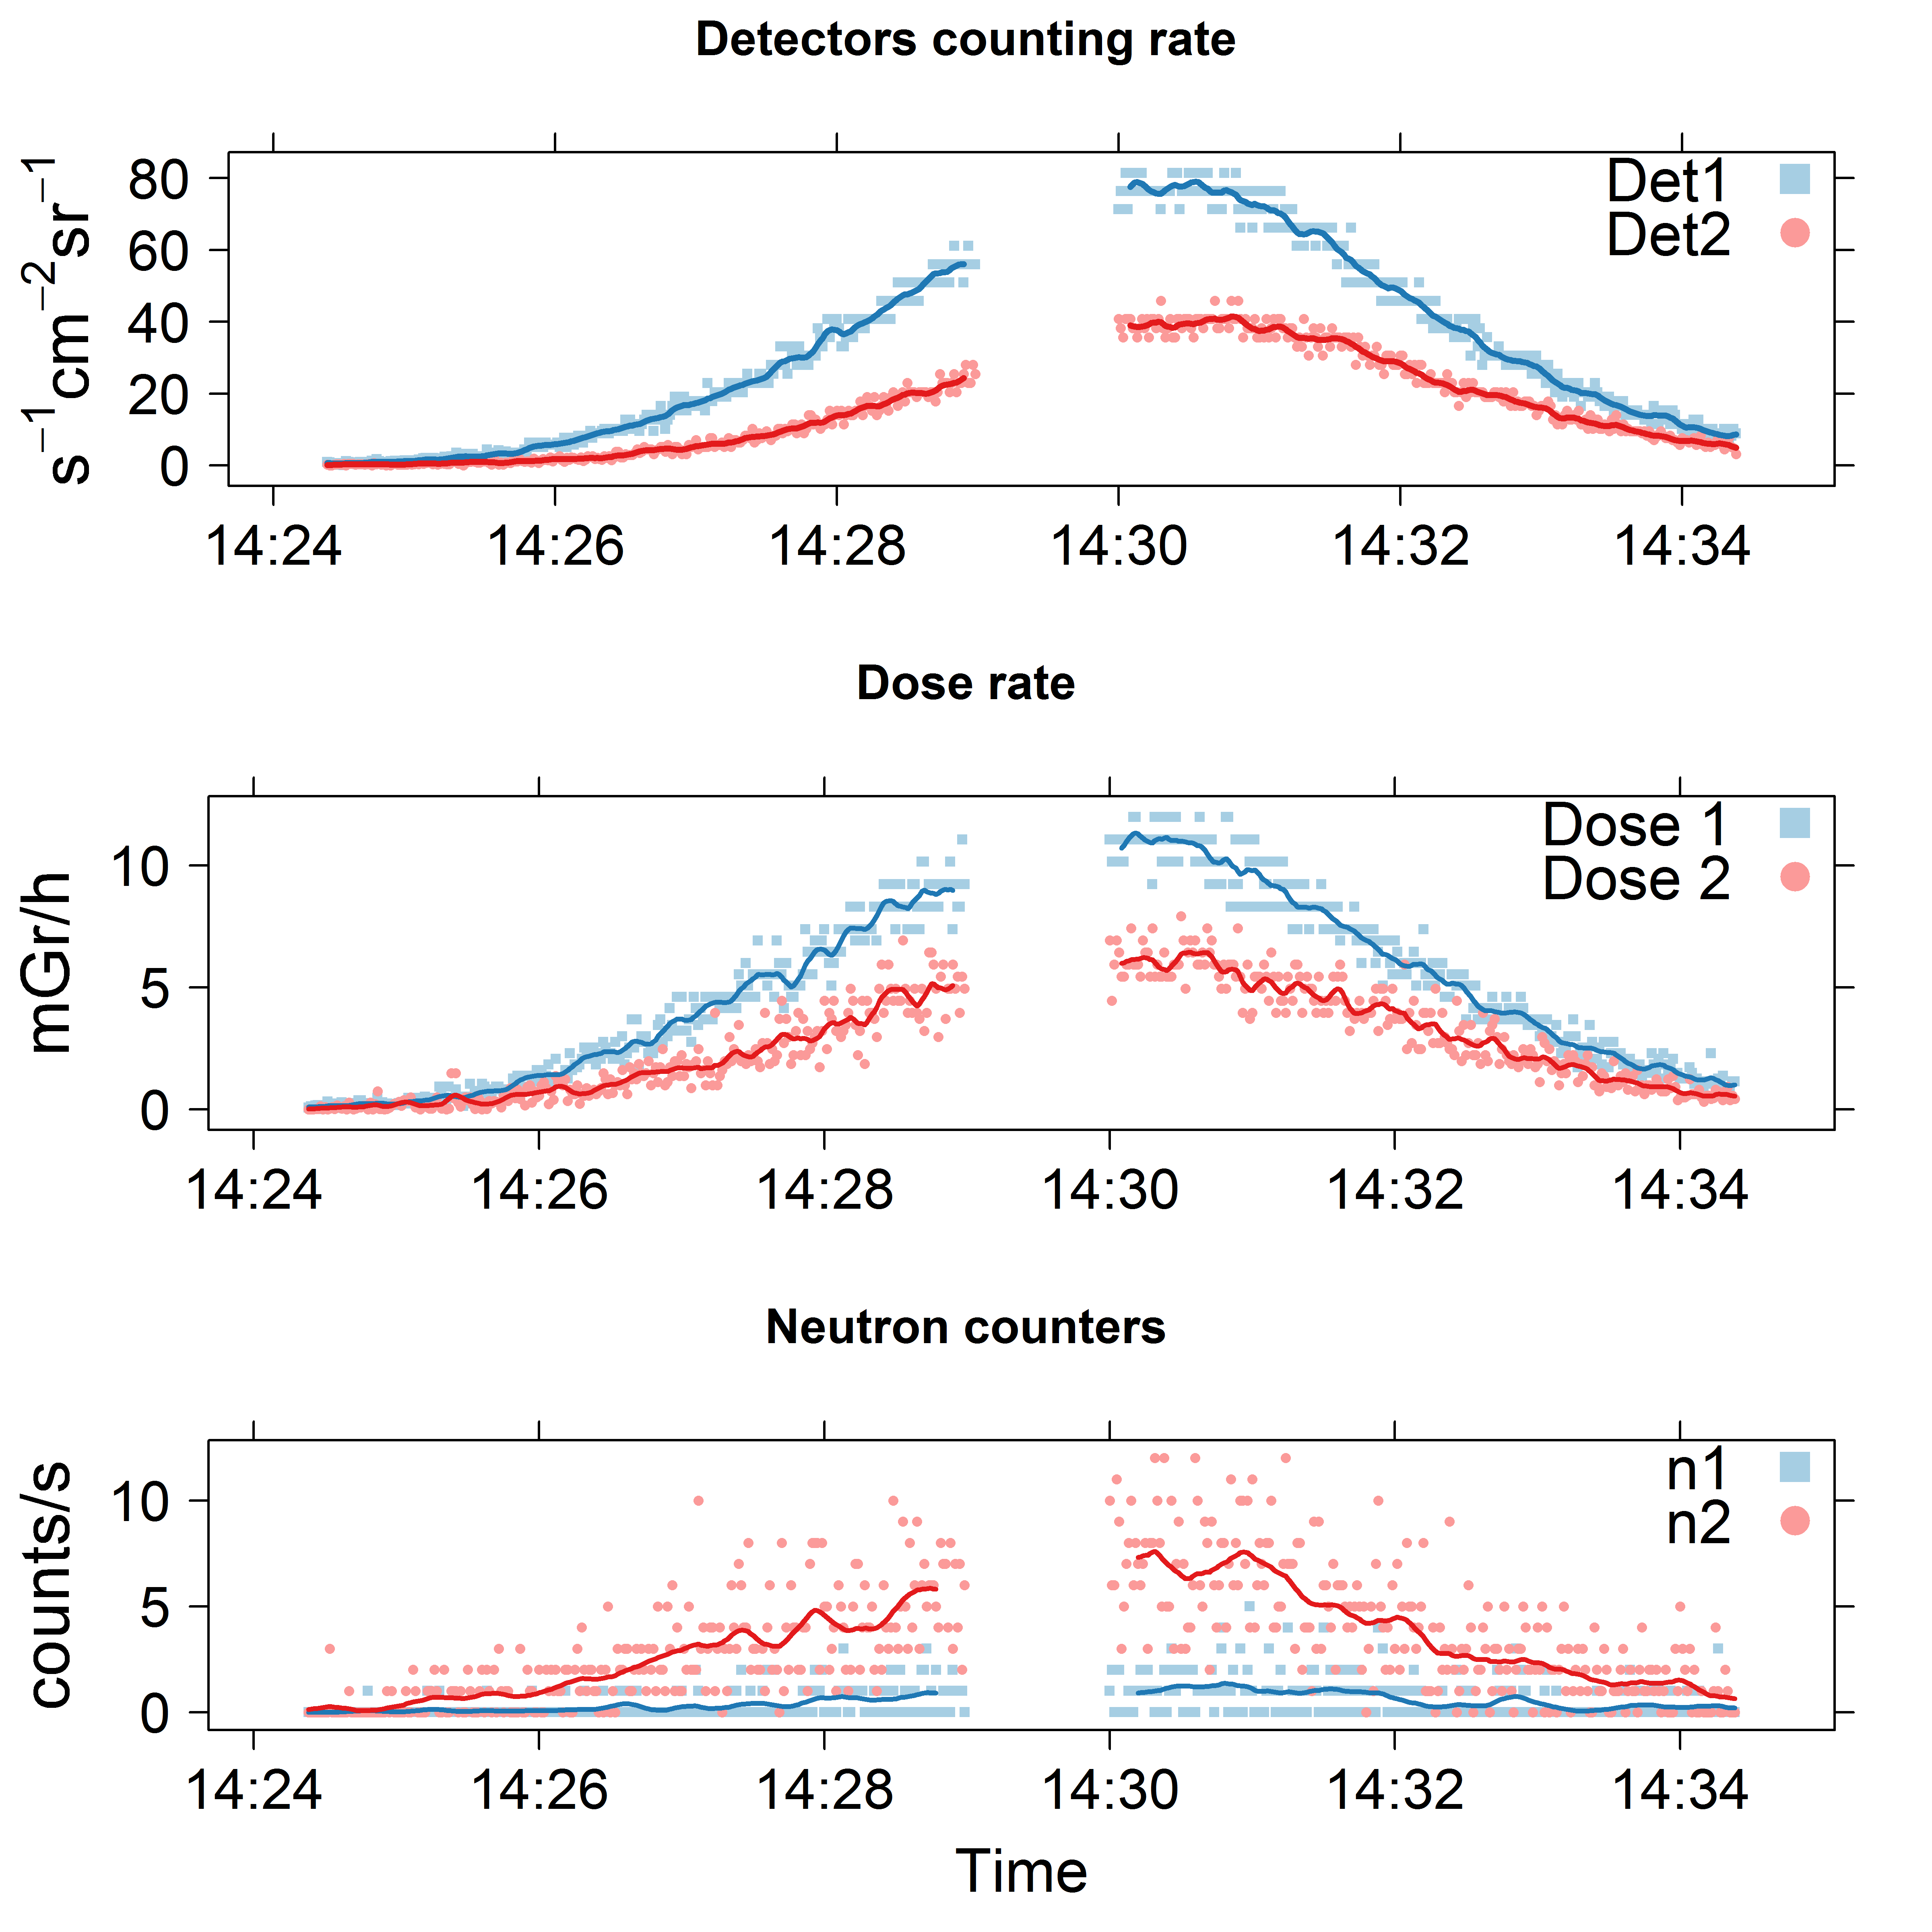
\includegraphics[width=0.7\linewidth]{images/results/depron_sec_log_new08-29-1614-24-23}
	\caption{}
	\label{fig:depronseclognew08-29-1614-24-23}
\end{figure}

\section{Распределение мощности дозы вне радиационных поясов Земли}

\section{Спектры ЛПЭ и распределение мощности эквивалентной дозы}